\documentclass{article}

\usepackage{tikz} 
\usetikzlibrary{automata, positioning, arrows} 

\usepackage{amsthm}
\usepackage{amsfonts}
\usepackage{amsmath}
\usepackage{amssymb}
\usepackage{fullpage}
\usepackage{color}
\usepackage{parskip}
\usepackage{hyperref}
\usepackage{graphicx}
  \hypersetup{
    colorlinks = true,
    urlcolor = blue,       % color of external links using \href
    linkcolor= blue,       % color of internal links 
    citecolor= blue,       % color of links to bibliography
    filecolor= blue,        % color of file links
    }
    
\usepackage{listings}
\usepackage[utf8]{inputenc}                                                    
\usepackage[T1]{fontenc}                                                       

\definecolor{dkgreen}{rgb}{0,0.6,0}
\definecolor{gray}{rgb}{0.5,0.5,0.5}
\definecolor{mauve}{rgb}{0.58,0,0.82}

\lstset{frame=tb,
  language=haskell,
  aboveskip=3mm,
  belowskip=3mm,
  showstringspaces=false,
  columns=flexible,
  basicstyle={\small\ttfamily},
  numbers=none,
  numberstyle=\tiny\color{gray},
  keywordstyle=\color{blue},
  commentstyle=\color{dkgreen},
  stringstyle=\color{mauve},
  breaklines=true,
  breakatwhitespace=true,
  tabsize=3
}

\newtheoremstyle{theorem}
  {\topsep}   % ABOVESPACE
  {\topsep}   % BELOWSPACE
  {\itshape\/}  % BODYFONT
  {0pt}       % INDENT (empty value is the same as 0pt)
  {\bfseries} % HEADFONT
  {.}         % HEADPUNCT
  {5pt plus 1pt minus 1pt} % HEADSPACE
  {}          % CUSTOM-HEAD-SPEC
\theoremstyle{theorem} 
   \newtheorem{theorem}{Theorem}[section]
   \newtheorem{corollary}[theorem]{Corollary}
   \newtheorem{lemma}[theorem]{Lemma}
   \newtheorem{proposition}[theorem]{Proposition}
\theoremstyle{definition}
   \newtheorem{definition}[theorem]{Definition}
   \newtheorem{example}[theorem]{Example}
\theoremstyle{remark}    
  \newtheorem{remark}[theorem]{Remark}

\title{CPSC-406 Report}
\author{Ethan Tapia  \\ Chapman University}

\date{\today} 

\begin{document}

\maketitle

\begin{abstract}
\end{abstract}

\setcounter{tocdepth}{3}
\tableofcontents

\section{Introduction}\label{intro}


\section{Week by Week}\label{homework}

\subsection{Week 1}
\textbf{Lecture Summary}

A finite automaton consists of a finite set of \textbf{states} ($Q$), an \textbf{alphabet} ($\Sigma$), a \textbf{transition function} ($\delta$), a \textbf{starting state} ($q_0$), and a set of \textbf{accepting states} ($F$). 

It can be formally represented as:

\[
M = (Q, \Sigma, \delta, q_0, F)
\]

where:
\begin{itemize}
    \item $Q$ is the set of states,
    \item $\Sigma$ is the input alphabet,
    \item $\delta: Q \times \Sigma \to Q$ is the transition function,
    \item $q_0 \in Q$ is the initial state,
    \item $F \subseteq Q$ is the set of accepting states.
\end{itemize}



\subsection{Week 2}
{\textbf{{Homework 1}}}

\textbf{Problem 1: Characterizing Accepted Sequences}

The given problem involves designing a finite automaton that accepts sequences of 5 and 10-cent inputs summing to 25 cents.

\textbf{Solution:}
We define the equation:
\begin{equation}
5a + 10b = 25
\end{equation}
where $a$ is the number of 5-cent inputs and $b$ is the number of 10-cent inputs. Solving for valid pairs:
\begin{itemize}
    \item $(a=5, b=0) \Rightarrow$ Sequence: $5,5,5,5,5$
    \item $(a=3, b=1) \Rightarrow$ Sequence: $5,5,5,10$
    \item $(a=1, b=2) \Rightarrow$ Sequence: $5,10,10$
\end{itemize}
These sequences are precisely those accepted by the automaton. The machine accepts a sequence if the total sum equals 25 cents.\newline

\textbf{Problem 2: Defining Valid Variable Names}

A valid variable name must begin with a letter ($\ell$) and be followed by any number of letters or digits ($d$).

\textbf{Regular Expression:}
\begin{equation}
\ell(\ell | d)^*
\end{equation}

\textbf{Solution:}
\textit{Finite Automaton:}
- States: $q_0$ (initial), $q_1$ (accepting).
- Transitions:
  - $q_0 \to q_1$ on input $\ell$
  - $q_1 \to q_1$ on input $\ell$ or $d$

\textbf{Problem 3: Classification of Words in $L_1, L_2, L_3$}

The given languages are defined as follows:

\begin{itemize}
    \item $L_1 = \{ x0y \mid x, y \in \Sigma^* \}$: The set of words that contain at least one '0'.
    \item $L_2 = \{ w \mid |w| = 2^n \text{ for some } n \in \mathbb{N} \}$: The set of words whose length is a power of 2.
    \item $L_3 = \{ w \mid |w|_0 = |w|_1 \}$: The set of words where the number of 0s equals the number of 1s.
\end{itemize}

\textbf{Solution:} We analyze each word based on these conditions:

\begin{table}[h]
    \centering
    \begin{tabular}{|c|c|c|c|}
        \hline
        & $L_1$ & $L_2$ & $L_3$ \\
        \hline
        $w_1 = 10011$ & \checkmark & \xmark & \xmark \\
        $w_2 = 100$ & \checkmark & \xmark & \xmark \\
        $w_3 = 10100100$ & \checkmark & \checkmark & \xmark \\
        $w_4 = 1010011100$ & \checkmark & \xmark & \checkmark \\
        $w_5 = 11110000$ & \checkmark & \checkmark & \checkmark \\
        \hline
    \end{tabular}
    \caption{Classification of words into $L_1, L_2, L_3$}
    \label{tab:language_classification}
\end{table}

\textbf{Problem 4: DFA Analysis}

Given the DFA with states $q_0$ (start), $q_2$, and $q_1$ (accepting), we determine which words end in the accepting state $q_1$.

\textbf{Transitions}:
\begin{align*}
    \delta(q_0, 1) &= q_0, & \delta(q_0, 0) &= q_2 \\
    \delta(q_2, 0) &= q_2, & \delta(q_2, 1) &= q_1 \\
    \delta(q_1, 0) &= q_1, & \delta(q_1, 1) &= q_1 \\
\end{align*}

\textbf{Checking Words}:
\begin{itemize}
    \item $w_1 = 0010$: $q_0 \to q_2 \to q_2 \to q_1 \to q_1$ \quad \checkmark (Accepted)
    \item $w_2 = 1101$: $q_0 \to q_0 \to q_0 \to q_2 \to q_1$ \quad \checkmark (Accepted)
    \item $w_3 = 1100$: $q_0 \to q_0 \to q_0 \to q_2 \to q_2$ \quad \xmark (Not Accepted)
\end{itemize}

\textbf{Solution:}

$w_1 = 0010$ \to \quad \checkmark \textit{Accepted} \\[0.3em]
$w_2 = 1101$ \to \quad \checkmark \textit{Accepted} \\[0.3em]
$w_3 = 1100$ \to \quad \xmark \textit{Rejected} 

This confirms that $w_1$ and $w_2$ end in the accepting state, while $w_3$ does not.


\textbf{Chapter 2.1 Report:}

Chapter 2.1 discusses the use of finite automata in modeling real-world protocols, particularly in the context of electronic money transactions. The section introduces a three-party system involving a customer, a store, and a bank. The goal is to ensure that digital money is not duplicated or reused fraudulently.

The protocol consists of five primary actions: pay, cancel, ship, redeem, and transfer. Each party's behavior is modeled using finite automata to track transaction states. The section highlights how such models can reveal vulnerabilities—such as a store shipping goods before verifying payment—showcasing the importance of automata in validating protocol security.

Finite automata prove to be useful for detecting logical flaws in transaction systems, ensuring valid sequences of operations. The chapter serves as an introduction to the application of formal computational models in the security and validation of protocols.

\subsection{Week 3}
\textbf{Lecture Summary}\\
%Summarize when I get the chance
\bigskip\bigskip\bigskip\bigskip\bigskip\bigskip\bigskip\bigskip\bigskip\bigskip\bigskip\bigskip\bigskip\bigskip\bigskip\bigskip\bigskip\bigskip\bigskip\bigskip\bigskip\bigskip\bigskip\bigskip\bigskip\bigskip\bigskip\bigskip\bigskip\bigskip

{\textbf{{Homework 2}}}\\
\textbf{Exercise 2: Implementing DFA Runs}\\
\begin{center}
\textbf{DFA $A_1$}
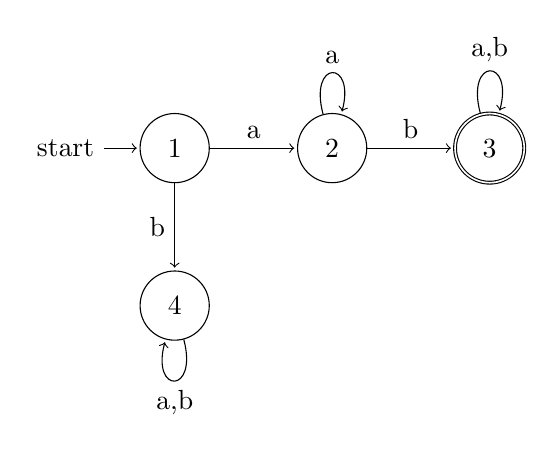
\begin{tikzpicture}[shorten >=1pt, node distance=2cm, on grid, auto] 

   \node[state, initial] (q1) {1}; 
   \node[state] (q2) [right=of q1] {2}; 
   \node[state, accepting] (q3) [right=of q2] {3}; 
   \node[state] (q4) [below=of q1] {4}; 

    \path[->]
    (q1) edge [above] node {a} (q2)
         edge [left]  node {b} (q4)
    (q2) edge [loop above] node {a} ()
         edge [above] node {b} (q3)
    (q3) edge [loop above] node {a,b} ()
    (q4) edge [loop below] node {a,b} ();
\end{tikzpicture}
\end{center}


\begin{center}
\textbf{DFA $A_2$}
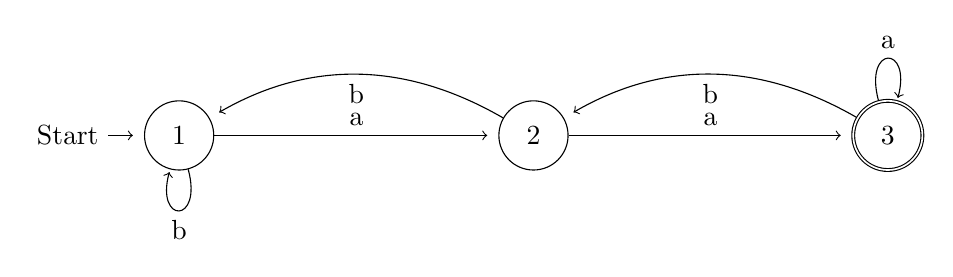
\begin{tikzpicture}[shorten >=4pt, node distance=4.5cm, on grid, auto] 

   \node[state, initial, initial text=Start] (q1) {1}; 
   \node[state] (q2) [right=of q1] {2}; 
   \node[state, accepting] (q3) [right=of q2] {3}; 

    \path[->]
    (q1) edge [above] node {a} (q2)
         edge [loop below] node {b} ()
    (q2) edge [above] node {a} (q3)
         edge [bend right=30, below] node {b} (q1)
    (q3) edge [loop above] node {a} ()
         edge [bend right=30, below] node {b} (q2);
\end{tikzpicture}
\end{center}


\textbf{Words accepted or refused by $\mathcal A_1$ and $\mathcal A_2$, respectively}
\[
\begin{array}{c|c|c}
w & \text{Accepted } A_1 & \text{Accepted } A_2 \\ \midrule
aaa & \textcolor{red}{\times} & \textcolor{green}{\checkmark} \\
aab & \textcolor{green}{\checkmark} & \textcolor{red}{\times} \\
aba & \textcolor{red}{\times} & \textcolor{red}{\times} \\
abb & \textcolor{red}{\times} & \textcolor{red}{\times} \\
baa & \textcolor{red}{\times} & \textcolor{green}{\checkmark} \\
bab & \textcolor{red}{\times} & \textcolor{red}{\times} \\
bba & \textcolor{red}{\times} & \textcolor{red}{\times} \\
bbb & \textcolor{red}{\times} & \textcolor{red}{\times} \\
\end{array}
\]
\noindent The table above summarizes the words accepted or rejected by DFA $A_1$ and DFA $A_2$. 
To implement these automata \textit{programmatically}, we define the DFA class in \texttt{dfa.py}, which allows us to process input words according to their respective state transition diagrams.

\textbf{\text{DFA Implementation in \texttt{dfa.py}}}\\
This introduction describes the design of the \texttt{dfa.py},  consisting of:
\begin{itemize}
  \item$Q$ - a finite set of states.
  \item$\Sigma$ - an input alphabet.
  \item$\delta : Q \times \Sigma \to Q$ - a transition function.
  \item$q_0 \in Q$ an initial state.
  \item$F \subseteq Q$ - a set of final accepting states.
\end{itemize}

The \texttt{DFA} class constructor takes these five elements (\texttt{Q}, \texttt{Sigma}, \texttt{delta}, \texttt{q0}, and \texttt{F}), using the method:
\begin{itemize}
  \item \texttt{run(w)}: Runs the DFA on input string \texttt{w} and determines whether or not \texttt{w} is accepted based on the state it finishes at.
\end{itemize}

\textbf{Implementation}
In the following code snippet, the \texttt{run} method processes the symbols of the input \texttt{w} sequentially, looking up the next state based on the current state and the input symbol. If an invalid transition is encountered, the method immediately returns \texttt{False}. Otherwise, if the DFA ends in a state that is a member of \texttt{F}, \texttt{True} is returned (meaning \texttt{w} is accepted); if it ends in some other state, \texttt{False} is returned.

\begin{lstlisting}
class DFA :

    # init the DFA
    def __init__(self, Q, Sigma, delta, q0, F) : 
        self.Q = Q # set of states
        self.Sigma = Sigma # set of symbols
        self.delta = delta # transition function
        self.q0 = q0 # initial state
        self.F = F # final states
   
   # print the data of the DFA
    def __repr__(self) :
        return f"DFA({self.Q},\n\t{self.Sigma},\n\t{self.delta},\n\t{self.q0},\n\t{self.F})"

    # run the DFA on the word w
    # return if the word is accepted or not
    # modify as needed
    def run(self, w) :
        # todo
        # start at initial state
        current_state = self.q0
        for symbol in w:
            if (current_state, symbol) in self.delta:
                current_state = self.delta[(current_state, symbol)]
            else:
                # invalid transition (dead state)
                return False
            # accept if in final state
        return current_state in self.F 

\end{lstlisting}

\textbf{Exercise 4: A new automaton from an old one}

Below is DFA $A_0$ which accepts exactly the words that $A$ refuses and vice versa.
\begin{center}
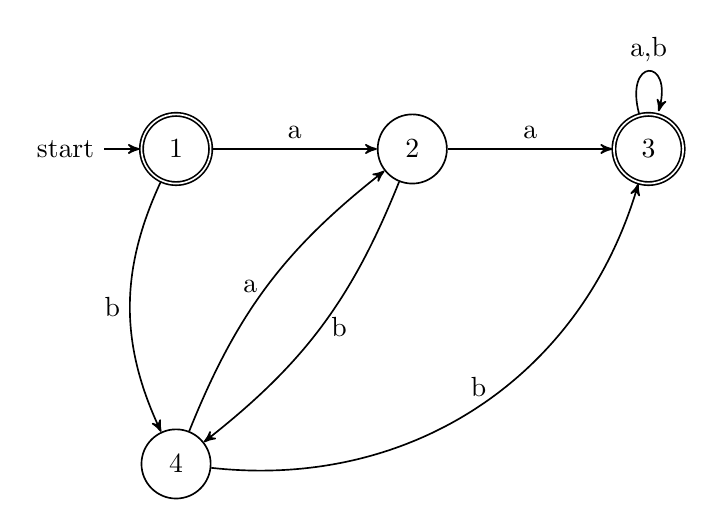
\begin{tikzpicture}[->, >=stealth', auto, semithick]
  \node[state, initial, accepting]      (q1) at (0,0)   {1};
  \node[state]                          (q2) at (3,0)   {2};
  \node[state, accepting]               (q3) at (6,0)   {3};
  \node[state]                          (q4) at (0,-4){4};
  \path
    % 1 -> 2, labeled 'a'
    (q1) edge                node[above] {a} (q2)
    % 1 -> 4, labeled 'b'
    (q1) edge[bend right=25] node[left]  {b} (q4)
    % 2 -> 3, labeled 'a'
    (q2) edge                node[above] {a} (q3)
    % 2 -> 4, labeled 'b'
    (q2) edge[bend left=15] node[right] {b} (q4)
    % 4 -> 2, labeled 'a'
    (q4) edge[bend left=15]  node[left]  {a} (q2)
    % 4 -> 3, labeled 'b'
    (q4) edge[bend right=40]  node[above] {b} (q3)
    % 3 -> 3 loop, labeled 'a,b'
    (q3) edge[loop above]    node        {a,b} ();

\end{tikzpicture}
\end{center}
In $A_0$, nodes 1 and 3 are the accepting final states, while nodes 2 and 4 are normal states.

\textbf{Exercise 2.2.4: DFAs over $\{0,1\}$}

{(a) The set of all strings ending in 00}

\noindent
\textbf{DFA Description:}
\[
\begin{aligned}
Q &= \{\,q_0,\, q_1,\, q_2\},\\
\Sigma &= \{0,1\},\\
\delta &\text{ is given by the table below},\\
q_0 &\text{ is the start state},\\
F &= \{\,q_2\}.
\end{aligned}
\]

\noindent
\textbf{Transition Table:}
\[
\begin{array}{c|cc}
  \delta & 0 & 1 \\
\hline
  q_0    & q_1 & q_0 \\
  q_1    & q_2 & q_0 \\
  q_2    & q_2 & q_0
\end{array}
\]

\noindent
\textit{Explanation:} 
\begin{itemize}
\item $q_0$ - we have not yet seen a trailing zero
\item $q_1$ - the string currently ends in exactly one zero
\item $q_2$ (accepting) - the string ends in at least two consecutive zeros
\end{itemize}

\bigskip

{(b) The set of all strings with three consecutive 0s}

\noindent
\textbf{DFA Description:}
\[
\begin{aligned}
Q &= \{\,q_0,\, q_1,\, q_2,\, q_3\},\\
\Sigma &= \{0,1\},\\
\delta &\text{ is given by the table below},\\
q_0 &\text{ is the start state},\\
F &= \{\,q_3\}.
\end{aligned}
\]

\noindent
\textbf{Transition Table:}
\[
\begin{array}{c|cc}
  \delta & 0 & 1 \\
\hline
  q_0    & q_1 & q_0 \\
  q_1    & q_2 & q_0 \\
  q_2    & q_3 & q_0 \\
  q_3    & q_3 & q_3
\end{array}
\]

\noindent
\textit{Explanation:}
\begin{itemize}
\item $q_0$ - we have seen 0 consecutive zeros so far
\item $q_1$ - we have seen exactly 1 consecutive zero
\item $q_2$ - we have seen exactly 2 consecutive zeros
\item $q_3$ (accepting) - we have seen at least 3 consecutive zeros
\end{itemize}

\bigskip

{(c) The set of all strings with \texttt{011} as a substring}

\noindent
\textbf{DFA Description:}
\[
\begin{aligned}
Q &= \{\,q_0,\, q_1,\, q_2,\, q_3\},\\
\Sigma &= \{0,1\},\\
\delta &\text{ is given by the table below},\\
q_0 &\text{ is the start state},\\
F &= \{\,q_3\}.
\end{aligned}
\]

\noindent
\textbf{Transition Table:}
\[
\begin{array}{c|cc}
  \delta & 0 & 1 \\
\hline
  q_0    & q_1 & q_0 \\
  q_1    & q_1 & q_2 \\
  q_2    & q_1 & q_3 \\
  q_3    & q_3 & q_3
\end{array}
\]

\noindent
\textit{Explanation:}
\begin{itemize}
\item $q_0$ - no partial match yet
\item $q_1$ - we matched a single \texttt{0}
\item $q_2$ - we matched \texttt{01}
\item $q_3$ (accepting) - we found \texttt{011} somewhere in the string
\end{itemize}


\end{document}


\section{Synthesis}

\section{Evidence of Participation}

\section{Conclusion}\label{conclusion}

\begin{thebibliography}{99}
\bibitem[BLA]{bla} Author, \href{https://en.wikipedia.org/wiki/LaTeX}{Title}, Publisher, Year.
\end{thebibliography}

\end{document}